\documentclass[11pt, oneside]{article}   	% use "amsart" instead of "article" for AMSLaTeX format
\usepackage{geometry}                		% See geometry.pdf to learn the layout options. There are lots.
\geometry{letterpaper}                   		% ... or a4paper or a5paper or ... 


\usepackage{graphicx}
\usepackage{setspace}				% Use pdf, png, jpg, or eps§ with pdflatex; use eps in DVI mode
								% TeX will automatically convert eps --> pdf in pdflatex		
\usepackage{amssymb}
\setlength{\parindent}{0em} 

%SetFonts

%SetFonts


\title{Physik E-Phase}
\author{The Author}

\doublespacing
\begin{document}
\maketitle

\pagebreak

\tableofcontents

\pagebreak

\section{Kinematik}
\subsection{Schr\"ager Wurf}



horizontal

$(h1)  s_x=v_{0,x}*t$

$(h2) v_x=v_{0,x}$

$(h3) a_x=0$

$v_x=konstant$

Da dies eine konstante Geschwindigkeit ist, d\"urfen wir die Formel

$s=v*t$

verwenden.

$s=v_{0,x}*2*(\frac{-v_0*sin(\alpha)}{g})$

$s_x=v_0*cos(\alpha)*2*(\frac{-v_0*sin(\alpha)}{g})$

$s_x=\frac{-v_0^2}{g}*2*cos(\alpha)*sin(\alpha)$

$s_x=\frac{-v_0^2}{g}*sin(2\alpha)$


vertikal

$(v1) s_y=v_{0,y}*t+\frac{1}{2}*g*t^2$

$(v2) s_y=v_{0,y}+g*t$

$(v3) a=g=-9,81\frac{m}{s^2}$



\pagebreak

\subsection{Aufgaben zum schr\"agen Wurf}

Metzler S. 31 / 4,6

Cornelsen

Aufgabe 14


a)

Maximale H\"ohe

$h_{max}=\frac{(-v_0)^2*(sin(\alpha))^2}{2g}$

\vspace{0.5cm}

Wurfweite

$s_x=\frac{-v_0^2}{g}*sin(2\alpha)$

\vspace{0.5cm}


Wurfzeit

$t_{max}=-\frac{(v_0)^2*(sin(\alpha))^2}{2g}$

\vspace{0.5cm}

b)

$t_{max}=-\frac{(v_0)^2*(sin(\alpha))^2}{2g}*\frac{v}{a}*s_0=-\frac{(9\frac{m}{s})^2*(sin(40�))^2}{2*9,81\frac{m}{s^2}}*\frac{9\frac{m}{s}}{9,81\frac{m}{s^2}}*1,80m=2,82s$

c)

\pagebreak

\section{Dynamik}

\subsection{Impuls}
Aus unserem Experiment folgt: $m_1*v_1=m_2*v_2$.

Die Gr\"osse $p=*v$ heisst Impuls. Der Impuls ist ein Ma� f\"ur den schr\"agen Wurf. Seine SI-Einheit ist $kg*\frac{m}{s}$. (englisch Impuls: momentum).

\pagebreak

\subsection{Der Impulserhaltungssatz}

In einem abgeschlossenen System ist die Summe der Impulse vor einem Stoss gleich der Summe der Impulse nach dem Stoss:

$p_1+p_2=p^1_1+p^1_2$

Eine r\"amliche begrenzte Aunordnung von K\"orpern, die nur untereinander in Wechselwirkung stehen, wird als, wird als abgeschlossen bezeichnet.

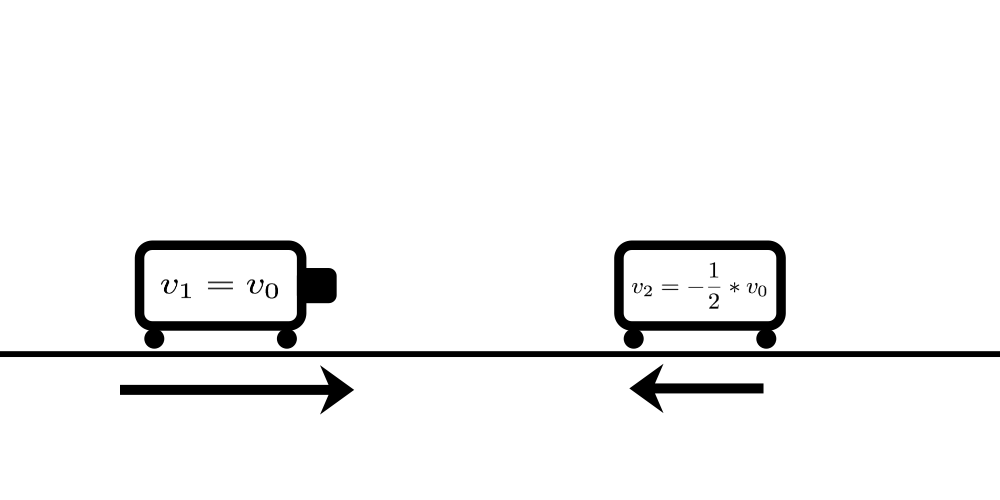
\includegraphics[width=0.5]{Wagen.png}


















\end{document}  